%! TEX root = ../main.tex
% ==============================================================
% IMMUTABLE — generated automatically, do not edit this block
%
% — Provenance ───────────────────────────────────────────────────
%   script            : analysis_scratch/plateau_overview.py
%   computed_in       : analysis_scratch/plateau_overview.py (sliding A_FFT, window N_off=7T, N_len=10T, step 0.1s, FFT band ±0.05 Hz)
%   plot_type         : plateau_overview
%   data_class        : DFS
%   generated_at      : 2026-04-30T12:50:40
%   findings_doc      : 
%
% — Thesis context ──────────────────────────────────────────────
%   chapter           : 04
%   caption_label     : fig:ch04_plateau_overview_A3
%   caption_short     : 
%
% — Filters ────────────────────────────────────────────────────
%   panel             : full
%   wind              : no, full
%   amplitude [V]     : 0.3
%   frequency [Hz]    : 
%   probes            : 
%   run_category      : 
%   quality_flag      : ok
%   mooring           : 
%
% — Data provenance ────────────────────────────────────────────
%   n_runs            : 25
%   in_probes_used    : 9373/170+9373/340
%   out_probes_used   : 12400/250
%   probe_configs     : march2026_better_rearranging
%   non_final_config_n: 
%   datasets        :
%     (none registered — set plot_utils.ACTIVE_DATASETS)
%   run_paths       :
%     (omitted — aggregate over > threshold runs, see datasets)
%
% — Method / numerical parameters ─────────────────────────────
%   grouper           : all canon runs at this (amp) — pooled per (f, wind, probe)
%   collapse_panels   : False
%   fft_window_hz     : 
%   extra_params      : target_amp = 0.3 V (A3); freqs = [1.3, 1.4, 1.5, 1.6]; r_IN = 9.373 m, r_OUT = 12.4 m; L_tank = 25.0 m; depth = 0.58 m; seiche speed = 2.385 m/s
%
% — Summary stats cited in caption ────────────────────────────
%   (none registered — pass extra_stats=... to build_fig_meta)
%
% — Subfigures available ───────────────────────────────────────
%     FIGURES/ch04_plateau_overview_A3.pdf
% ── end immutable block ─────────────────────────────────────────
\begin{figure}[htbp]
  \centering
  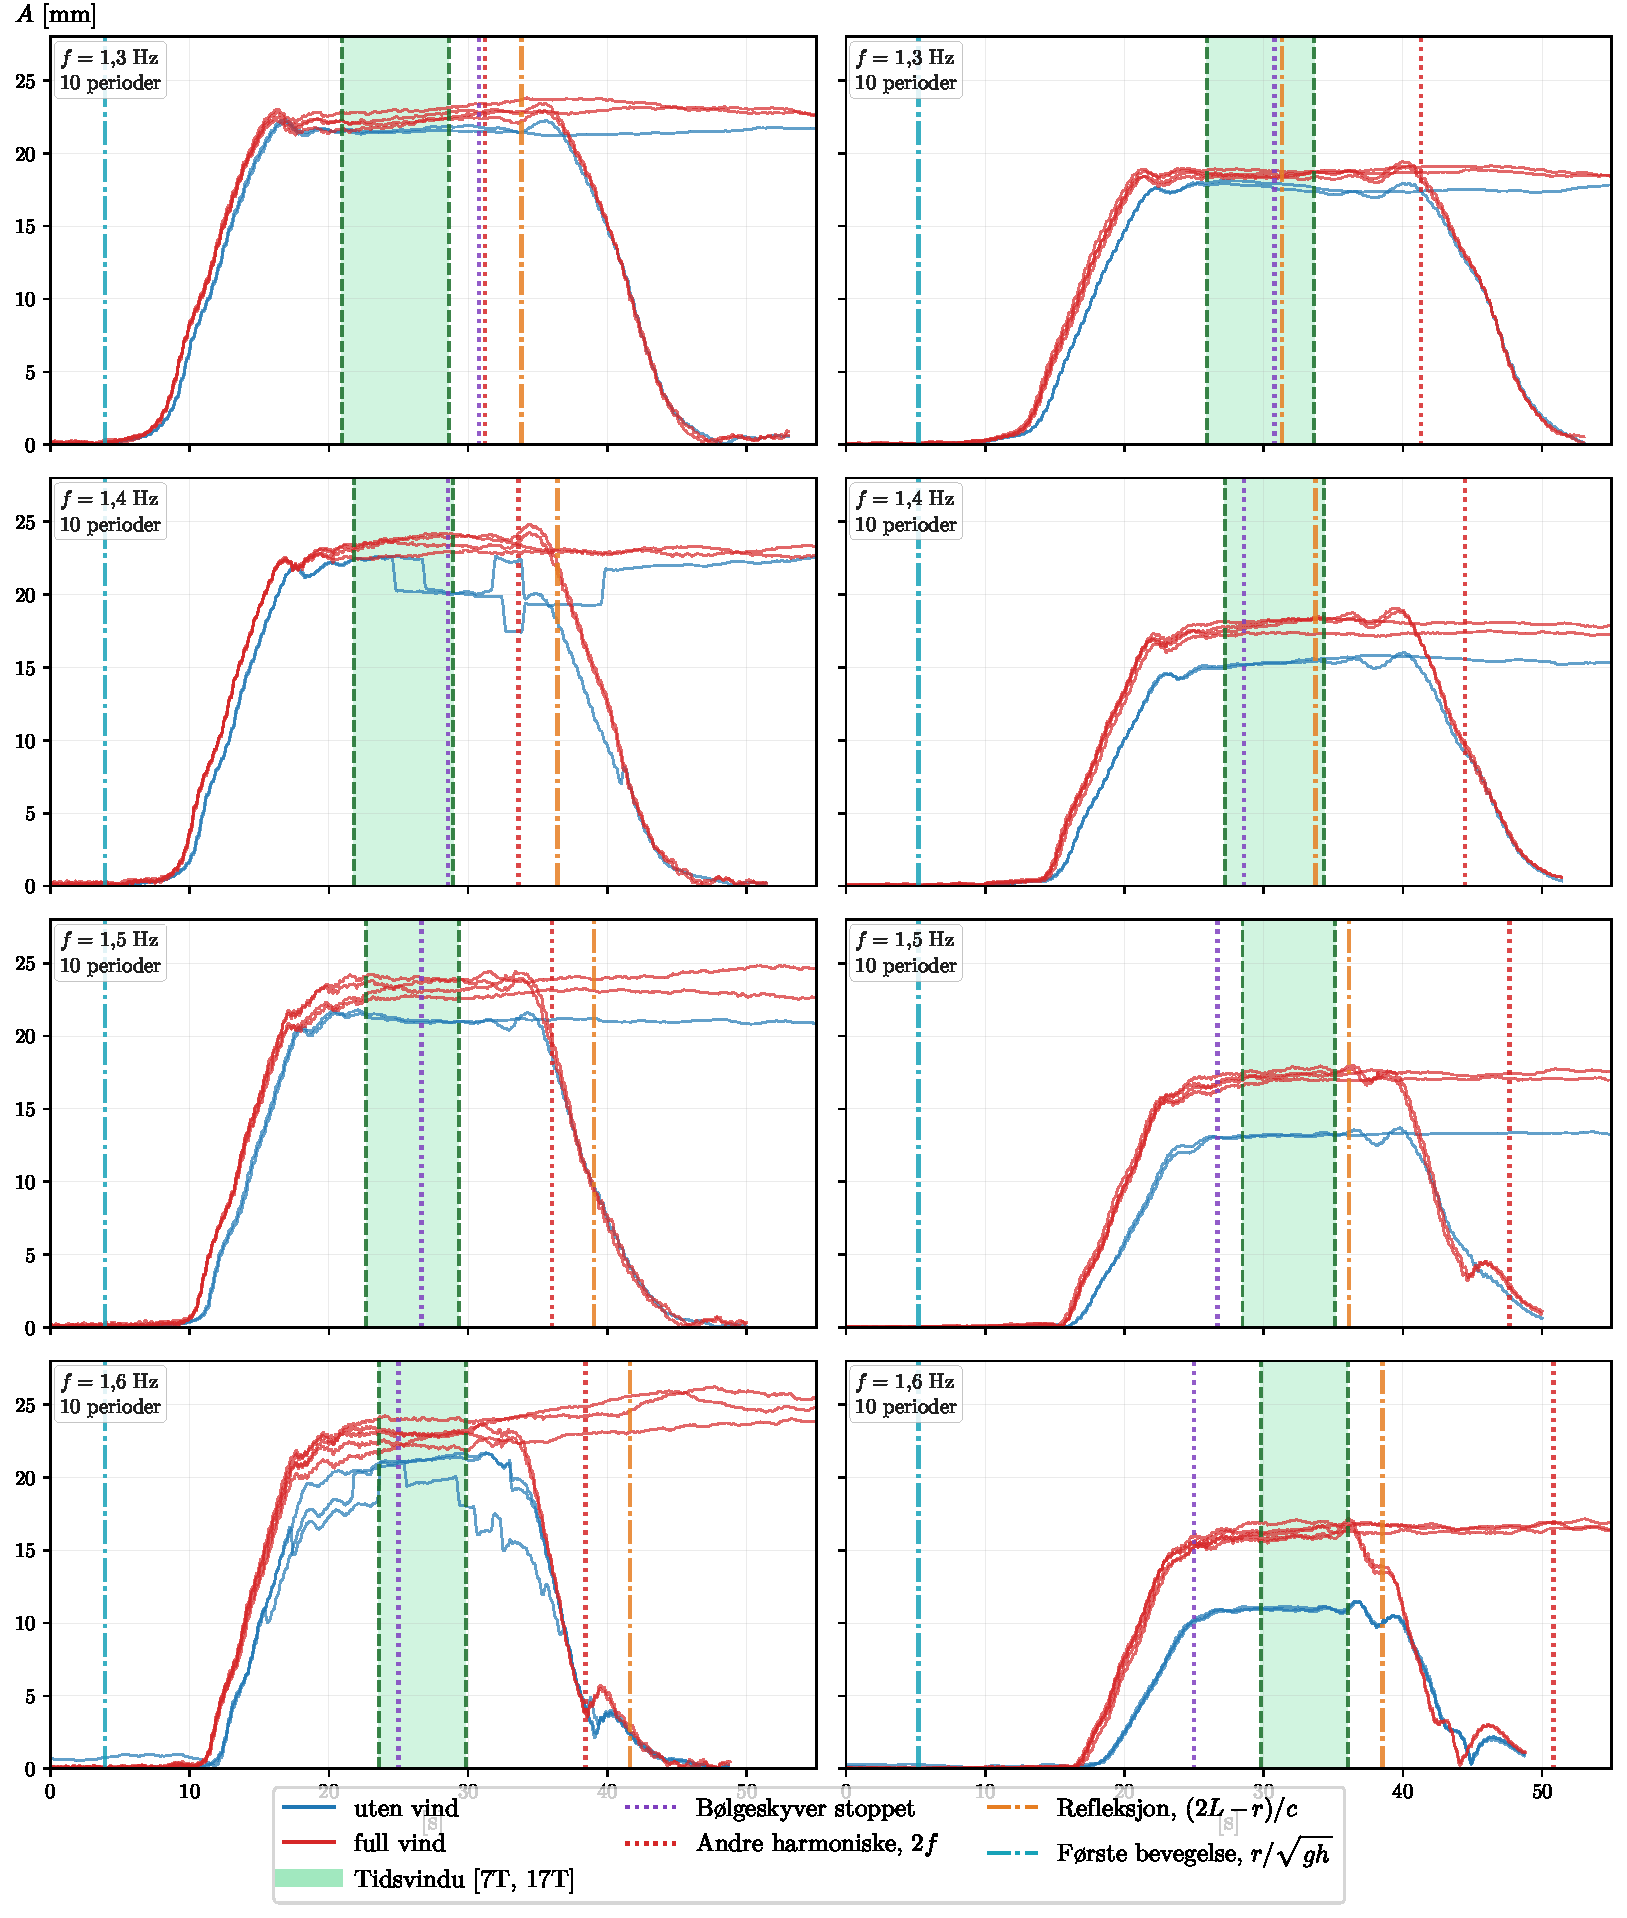
\includegraphics[width=\linewidth]{FIGURES/ch04_plateau_overview_A3.pdf}
  \caption{
    % TODO: write caption
  }
  \label{fig:ch04_plateau_overview_A3}
\end{figure}
